%---------- Quinto Capítulo ----------
\chapter{Análise de Segurança e Desempenho}

Com a definição da arquitetura de referência REST e do protocolo de autenticação e autorização (Capítulo~\ref{cap:Protocolo}), tornou-se necessária a realização de uma análise de segurança e de experimentos que possibilitam a mensuração do impacto da sua utilização no tratamento das requisições realizadas à PCDF.

Este capítulo inicialmente apresenta uma análise dos mecanismos de segurança propostos no protocolo. Essa primeira
análise segue um procedimento informal, mas está de acordo com trabalhos descritos na literatura~\cite{} {\color{red}citar
disserta\c c\~{o}es, teses e artigos que fazem uma an\'{a}lise similar.}. Em seguida, este capítulo apresenta uma avaliação empírica que busca analisar o desempenho do protocolo de Autenticação e Autorização Proposto.

\section{Análise de Segurança}

Nesta seção serão discutidas as propriedades de segurança do protocolo de autenticação e autorização proposto. São abordadas as propriedades e alguns ataques que podem ser realizados. Essa seção segue a estrutura e se fundamenta (parcialmente) no discurso utilizado na análise do protocolo Traust~\cite{traust08}.

\subsection{Segurança da sessão}

O protocolo de Autenticação e Autorização proposto utiliza para segurança de sessão e camada de transporte, o protocolo TLS/SSL. A utilização desse protocolo tem por objetivo evitar o ataque \emph{man-in-the-middle}. Para isso, é exigido, tanto para o órgão conveniado quanto para a própria PCDF, a utilização de certificados digitais padrão X.509, emitidos e garantidos por uma CA que esteja subordinada à hierarquia da ICP-Brasil.

Com isso, ambas as partes envolvidas no processo de comunicação podem estabelecer um processo de confiança mútua no nível de transporte. Todo o tráfego que flui sobre uma sessão bilateral certificada tem uma fonte confiável. Isso permite que implementações de serviços possam autorizar ou desautorizar interações com base na fonte bem conhecida de uma solicitação HTTP.

Além da segurança oferecida pela utilização da segurança na camada de transporte, com utilização do TLS/SSL, o protocolo utiliza mecanismos de segurança tais como criptografia assimétrica e assinatura digital. Isso Permite que outras partes mal intencionadas não consigam ter acesso ao conteúdo das mensagens trocadas pelo protocolo no processo de comunicação.

Diferentemente do sistema Traust~\cite{traust08}, o protocolo de Autenticação e Autorização proposto, será executado apenas em ambientes que tanto o cliente quanto o servidor possuem chaves públicas certificadas. Procura-se, dessa forma, atenuar problemas relacionados ao protocolo TLS, que quando executado em ambientes em que as partes
n\~{a}o possuem chaves públicas certificadas, relacionados a ataques \emph{man-in-the-middle} durante o estabelecimento da sessão~\cite{traust08}.

\subsection{Responsabilização dos usuários conveniados}

Uma das ameaças verificadas diz respeito a possibilidade do uso indevido, por parte dos órgãos conveniados, das informações disponibilizadas nos serviços ofertados pela PCDF. Isso decorre porque as informações disponibilizadas s\~{a}o sensíveis e possuírem caráter sigiloso. Dessa forma, para evitar esse problema é exigido dos órgãos conveniados que assinem um contrato para o consumo do serviço. No momento da assinatura do contrato as institui\c c\~{o}es recebem uma tabela contendo várias credenciais que servem como identidade e que deverão ser utilizadas no processo de autenticação, conforme descrito no seção~\ref{sec:reqprotocolo}. Isso possibilita que ocorra uma autenticação mútua entre a PCDF e os consumidores dos serviços. Além disso, com a utilização do protocolo de autenticação e autorização proposto, são empregados mecanismos de criptografia e assinaturas digitais que são geradas a partir de certificados digitais padrão X.509 vinculados aos órgãos e garantidos por AC. Dessa forma, busca-se evitar o não-repúdio por parte das instituições conveniadas,atribuindo-lhes responsabilidades em caso do mau uso dos serviço ofertados pela PCDF. Logo, uma vez detectado algum tipo de vazamento de dados proveniente dos serviços ofertados o órgão poderá ser identificado e após uma apuração minuciosa, responsabilizado pelos danos causados à PCDF.

\subsection{Ataques de repetição}

Esta ameaça, conforme descrita na Seção~\ref{sec:vulnerabilidadessoa}, se empregada contra o protocolo de autenticação e autorização proposto, tem baixa probabilidade de sucesso. Isso porque utilizamos \emph{timestamps} na maior parte das mensagens trocadas pelo protocolo. Além disso, são gerados números únicos, que identificam os desafios de autenticação gerados e que podem ser utilizados como \emph{nonces}, valores gerados de forma aleat\'{o}ria e que podem ser empregados contra esse tipo de ataque.

\subsection{Ataques de negação de serviço}

Esta ameaça é muito difícil de ser evitada, uma vez que  pode ser fruto de ataques via rede, do consumo excessivo de recursos da máquina  ou, ainda, ser resultante da exploração de qualquer tipo de vulnerabilidade que implique na indisponibilidade do serviço ou de um recurso. O protocolo de autenticação e autorização proposto é baseado no esquema de desafio-resposta. Os desafios são gerados de forma aleatória a partir das credenciais que identificam unicamente os consumidores dos serviços, o que possibilita uma autenticação mútua. Além disso, também são empregados outros mecanismos de segurança como utilização da segurança na camada de transporte e mecanismos de criptografia e assinaturas digitais. Isso minimiza a ameaça de ataques de negação de serviço. Assim como o protocolo Traust~\cite{traust08}, o servidor de autenticação e autorização proposto pode ser replicado para outros servidores, o que possibilita um balanceamento de carga e minimiza a criação de gargalos. Isso permite que o servidor de autenticação seja escalável e esteja disponível em situações críticas, como no caso dos ataques de negação de serviço.


\subsection{Roubo de credenciais de autenticação e autorização}\label{subsec:RouboCred}

O protocolo de autenticação a autorização proposto, após executado corretamente, emite um token de segurança que será utilizado para a obtenção do serviço desejado, conforme apresentado na seção~\ref{sec:ArqProtocolo}. Cabe ressaltar que se um atacante conseguir burlar os mecanismos de segurança utilizados pelo protocolo e conseguir acesso a essa credencial de autenticação e autorização, o atacante terá acesso apenas um serviço, pois o protocolo emite credenciais para um único serviço por vez e com tempo de expiração determinado no momento de sua geração. Essa é uma situação muito difícil de ser verificada, porém caso o extravio de credenciais ocorra, buscamos minimizar o problema com o
isolamento de uma credencial por servi\c co requisitado, diminuindo o impacto que pode ocorrer.

Outro problema que pode ocorrer é o roubo de credenciais de autenticação, que são as credenciais que o órgão conveniado recebe no momento da assinatura do contrato de oferecimento do serviço. Essa credenciais são utilizadas para responder aos desafios que serão realizadas pelo protocolo de autenticação proposto. Caso o extravio o ocorra e seja identificado, a PCDF pode, de forma flex\'{i}vel e transparente, desativar as credenciais que julga terem sido comprometidas sem que o usuário seja prejudicado.
Em um caso mais extremo, outras credenciais podem ser geradas e redistribuídas \`{a}s institui\c c\~{o}es conveniadas.

Porém, cabe ressaltar que, caso ocorra o extravio de credenciais, o órgão que teve o problema será investigado e poderá ser responsabilizado--- caso seja detectada uma m\'{a}
gestão na guarda das credenciais, conforme descrito na subseção~\ref{subsec:RouboCred}


\subsection{Ponto único de ataque}

Uma das possibilidades verificadas é que, ocorrendo um ataque, o alvo possa não ser protocolo de autenticação e autorização proposto e sim o próprio \servidorAA.
Neste caso, se o atacante for bem sucedido o servidor poder ficar vulnerável. Esse servidor é responsável pela geração dos desafios de autenticação e pela geração das credenciais de autenticação e autorização. Porém, apesar de realizar estas atividades ele armazena e consulta os dados gerados no processo de autenticação e autorização em outra máquina, que é em um servidor de banco de dados. Em outras palavras, o \servidorAA está em uma máquina diferente do servidor de banco de dados, o que minimiza os problemas relacionados a esse tipo de ataque, pois o servidor pode ser replicado para outra máquina e o que estiver com problemas pode ser facilmente substituído.

\subsection{S\'{i}ntese da an\'{a}lise de seguran\c ca}

\begin{itemize}
\item descrever os pontos positivos
\item descrever os pontos que requerem mais aten\c c\~{a}o
\end{itemize}

\section{Testes de desempenho}

Testes de desempenho são definidos como investiga\c c\~{o}es técnicas realizadas 
para determinar a capacidade de resposta, a confiabilidade ou escalabilidade de um sistema, 
sob uma determinada carga de trabalho~\cite{Meier2007}.
A análise de desempenho possibilita identificar problemas que geralmente são encontrados em sistemas computacionais. 
Esses problemas podem ser agrupados em termos de comparação e configuração de sistemas, identificação de gargalos, 
caracterização de cargas de trabalho e a previsão de desempenho~\cite{jain1991art}. Dessa forma, foram conduzidos 
experimentos com o objetivo de analisar o desempenho do protocolo de autenticação e autorização proposto. O restante 
dessa se\c c\~{a}o descreve os procedimentos e os resultados obtidos com a an\'{a}lise de desempenho. 
 
\subsection{Objetivos, Questões e Métricas}\label{sec:gqm}

A avaliação de desempenho do protocolo de autenticação e autorização proposto foi organizada com o uso da abordagem 
GQM (\emph{Goals, Questions, and Metrics})~\cite{gqm}. O resultado da aplicação da GQM é a especificação de um sistema de 
medição visando um conjunto particular de problemas e um conjunto de regras para a interpretação dos dados de medição~\cite{gqm}.  
O modelo de avaliação resultante tem três níveis: nível conceitual, onde  são definidos os objetivos da medição; nível operacional, que é aquele 
onde são verificadas as questões  que caracterizam o objeto da medição; e o nível quantitativo, que é o nível onde são definidas as métricas que 
identificam a medidas necessárias para responder as questões levantadas~\cite{gqm}. 

\subsubsection{Objetivos }\label{sec:gqmobjetivos}

A realização de testes de desempenho objetivam determinanr  se o desempenho de um algoritmo, protocolo ou sistema está de acordo com os requisitos. 
Outro objetivo dos testes de desempenho é o de validar a capacidade de resposta, a vazão, a confiabilidade e a escalabilidade de um sistema sob 
uma determinada carga~\cite{Meier2007}. Em rela\c c\~{a}o ao trabalho desenvolvido nessa disserta\c c\~{a}o, 
a avaliação de desempenho do protocolo de autenticação e autorização proposto tem como objetivo:

\begin{itemize}
\item Verificar o impacto do protocolo de autenticação e autorização proposto;
\item Identificar a viabilidade do uso do protocolo em cen\'{a}rios de carga esperados para a PCDF.
\end{itemize}


\subsubsection{Questões}\label{sec:gqmquestoes}

Seguindo o que é preconizado na metodologia GQM, os objetivos são definidos em um nível abstrato, de forma que devem ser formuladas questões, em um nível operacional, que têm por finalidade responder se os objetivos definidos serão atendidos. Logo, com base nos objetivos formulados para a análise de desempenho do protocolo de autenticação e autorização 
proposto, as seguintes questões foram investigadas:

\parbox{0.8\textwidth}{
\begin{enumerate}[(Q1)]
\item \emph{Qual o impacto observado no tempo de resposta às requisições com o uso do protocolo?}
\item \emph{Um protótipo funcional, sem foco em otimização, consegue suportar a demanda prevista?}
\end{enumerate}}

\subsubsection{Métricas}

O desempenho é descrito quantitativamente por meio de métricas. Uma métrica pode ser definida como um conjunto de dados que é definido para responder uma questão de maneira quantitativa. Dessa forma, foram utilizadas as seguintes métricas na avaliação do desempenho do protocolo de autenticação e autorização proposto. 

\begin{itemize}
\item quantidade de usuários: vari\'{a}vel de controle que representa a quantidade de usuários utilizados na avaliação de desempenho.

\item utilização do protocolo: vari\'{a}vel de controle que indica a utiliza\c c\~{a}o ou n\~{a}o do protocolo proposto na disserta\c c\~{a}o. Ela é definida em dois níveis, SIM ou  NÃO.

\item tempo médio de resposta: vari\'{a}vel de resposta que consiste no tempo entre a solicitação de um serviço por um usuário até o momento em que ele recebe uma resposta 
completa~\cite{ Molyneaux2009}. Para a análise de desempenho do protocolo proposto o tempo médio será dado em milissegundos.

\item Vazão (\emph{throughput}): vari\'{a}vel de resposta que corresponde ao número de operações que podem ser tratadas pelo protocolo em um 
determinado período de tempo~\cite{ Molyneaux2009}.

\end{itemize}

Dessa forma, após definir as métricas utilizadas na avaliação de desempenho, foi criado um plano de medição que descreve 
como as vari\'{a}veis de resposta serão mensuradas e quais procedimentos ser\~{a}o realizados 
durante o período de execução dos experimentos.

Logo, o primeiro passo foi a criação de um serviço REST, que retorna informações sobre ocorrências policiais, tais como: 
quais tipos de ocorrências criminais estão registradas, dados gerais da vítima, autor, dentre outras informações. 
Esse serviço é consumido  no momento da execução dos testes de desempenho da solução proposta. 
Foram realizados 10 cen\'{a}rios de testes, conforme representado na Tabela~\ref{tb:tb_testes}.

\begin{table}[h]
\begin{center}
\begin{tabular}{|c|c|c|}
\hline
N. de usuários & Sem utilização do protocolo & Com utilização do Protocolo \\ \hline
10             & Teste 1                     & Teste 2                     \\ \hline
20             & Teste 3                     & Teste 4                    \\ \hline
30             & Teste 5                     & Teste 6                    \\ \hline
40             & Teste 7                     & Teste 8                    \\ \hline
50             & Teste 9                     & Teste 10                    \\ \hline
\end{tabular}
\caption {Cen\'{a}rios de testes realizados}\label{tb:tb_testes}
\end{center}
\end{table}

Para a execução dos testes, que utilizam as métricas definidas, foram estabelecidas as seguintes regras: Cada teste deve realizar várias requisições ao serviço REST 
criado e o número de requisições é obtido pela fórmula $numeroUsuarios \times 100$. A frequência de lançamento das threads, 
que representam os usuários virtuais, é definido pela fórmula $numeroUsuarios \times 2s$. Exemplificando, 
de acordo com a Tabela~\ref{tb:tb_testes}, ao selecionar o Teste 1, serão executadas 10 threads a cada 20 segundos. 
Importa salientar que cada thread corresponde a um usuário, é iniciada 2 segundos após a thread anterior e executa 100 requisições---
o que totaliza 1000 requisições ao serviço no cen\'{a}rio Teste 1. Esse procedimento foi adotado para os demais cen\'{a}rios de testes. 
Por fim, as variáveis de resposta adotadas para a análise de desempenho, conforme discutido, 
foram o tempo médio de resposta das requisições e a vazão média de requisições por segundo.

\subsection{Configuração do ambiente de teste}

O ambiente de teste envolveu estações de trabalho tanto do Laboratório de Engenharia de Software da Universidade de Brasília quanto na 
Divisão de Tecnologia da Policia Civil do Distrito Federal. Para a realização dos testes foram 
utilizadas configurações distintas de computadores, conforme apresentado na tabela~\ref{tb:estudo_caso1}.

\begin{table}[h]
\begin{center}
    \begin{tabular}{|p{6cm}|c|p{6cm}|}
    \hline
    Esta\c c\~{a}o                  & Quantidade & Configura\c c\~{a}o \\ \hline
    Servidor de Autenticação e Autorização     & 1          & Desktop DELL Intel Core I5-2450 2,5 GHz, 4 Gb RAM, 500 HD \\ \hline
    Servidor de Fachada REST                   & 1          & Desktop DELL Intel Core I5-2450 2,5 GHz, 4 Gb RAM, 500 HD \\ \hline
    Cliente REST                               & 1          & Desktop DELL Intel Core I5-2450 2,5 GHz, 4 Gb RAM, 500 HD \\ \hline
    Servidor do Serviço web REST PCDF       & 1          & Intel Xeon E7 4870 2,4 GHz, 8 Gb RAM, 120 HD \\ \hline
    \end{tabular}
    \caption {Ambiente utilizado na análise de desempenho}\label{tb:estudo_caso1}
\end{center}
\end{table}

Os servidores de Autenticação e Autorização, Fachada REST e Cliente REST, foram prototipados utilizando a linguagem de programação funcional \emph{Haskell}. Estes 
servidores acessam uma base de dados não relacional \emph{CouchDB}, conforme apresentado na seção~\ref{sec:implementacao}. 
O sistema operacional utilizado nessas máquinas foi o Linux Ubuntu 12.04 LTS-64 bits. No caso do serviço REST desenvolvido pela PCDF, 
para atender a demanda da análise de desempenho, foi desenvolvido utilizando a linguagem C\# acessando um banco de dados \emph{SQL Server 2008 r2} 
que mant\'{e}m os registros das ocorr\^{e}ncias policiais. O serviço foi publicado em um servidor que utiliza o sistema operacional 
\emph{Windows Server 2008 r2, Enterprise Edition x64}, utilizando o ISS 7.0 como servidor Web. 
A Figura~\ref{fig:ambiente_teste} descreve os ambientes de configuração utilizados na análise de desempenho do {\color{red}(tem que padronizar. em 
alguns pontos est\'{a} mai\'{u}sculo, em outros min\'{u}sculo)Protocolo de Autenticação e Autorização proposto}.


\begin{figure}[!htb]
\centering
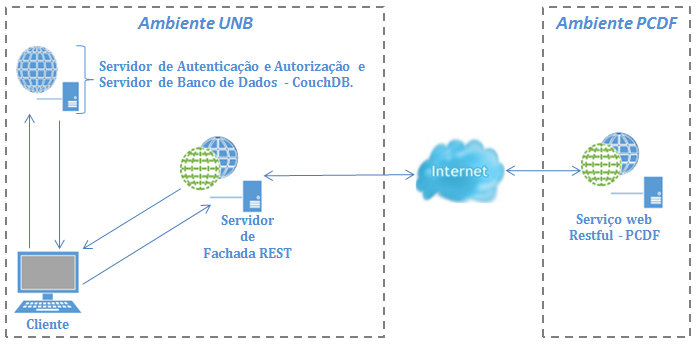
\includegraphics[width=0.8\textwidth]{ambiente_teste_desempenho.png}
\caption{Ambiente de teste de desempenho do Protocolo de Autenticação e Autorização.}
\label{fig:ambiente_teste}
\end{figure}

\subsection{Análise dos resultados}

Os testes objetivam (a) verificar o impacto no tempo de resposta às requisições com o uso do protocolo e (b) avaliar se um protocolo funcional, sem foco em otimização, 
suportaria a demanda de requisi\c c\~{o}es prevista para a PCDF. Para atender aos objetivos supracitados, foram realizados testes considerando 
requisi\c c\~{o}es diretas, sem o uso do protocolo de autentica\c c\~{a}o e autoriza\c c\~{a}o; e requisi\c c\~{o}es seguras e que seguem as trocas 
de mensagens definidas no protocolo. Conforme discutido nas se\c c\~{o}es anteriores, as an\'{a}lises resultaram em um universo de amostras
com 1000, 2000, 3000, 4000 e 5000 requisi\c c\~{o}es, correspondendo respectivamente a grupos de 10, 20, 30, 40 e 50 usuários. 
Os dados coletados foram analisados, e resultados estatísticos são apresentados nas  tabelas~\ref{tb:estatistica_com_cripto} e ~\ref{tb:estatistica_sem_cripto}. 

Dessa forma, com o objetivo de responder a primeira questão relacionada ao teste de performance 
(\emph{Qual o impacto observado no tempo de resposta às requisições com o uso do protocolo?}), 
consideramos que os resultados obtidos evidenciam um impacto significativo com a utilização do protocolo de autenticação e autorização proposto. 
Pode-se observar que, com a utilização do protocolo para 10 usuários simultâneos, o tempo médio de resposta é de 683,84 milissegundos. 
Por outro lado, quando comparado ao acesso ao serviço sem a utilização do protocolo, o tempo médio de resposta às requisições é de 42,26 milissegundos. 
Estas comparações estendem-se aos demais cen\'{a}rios de testes, para 20, 30, 40 e 50 usuários. Em todos casos o impacto é significativo quando comparado 
aos resultados obtidos sem a utilização do protocolo de autenticação e autorização. Porém, essa variação era de certa forma esperada, pois o protocolo proposto 
incorpora mecanismos de segurança que requerem algoritmos de criptografia e assinatura digital e segurança na camada de transporte com a utilização do SSL/TLS. 
Além disso, a implementação do protocolo será ainda alvo de otimizações.

De outra forma, ao analisar o tempo médio dos experimentos que utilizaram o protocolo, nota-se que este tempo é aceitável, pois com 10 usuários ele fica abaixo de 1 segundo, com 20 o tempo médio é 1,5 segundos, com 30 usuários esse tempo sobe para aproximadamente 2,5 segundos, aumentado de forma aceitável até 50 usuários em que o tempo médio verificado foi de aproximadamente 4,5 segundos, conforme apresentado nas tabelas ~\ref{tb:estatistica_com_cripto} e ~\ref{tb:estatistica_sem_cripto} e no gráfico ~\ref{fig:grafico_teste_desempenho}. De forma que esses resultados estão dentro do esperado para utilização. Atualmente o número de convênios na PCDF não supera 10 usuários, estima-se que com a utilização do protocolo esse número suba para no máximo 30 órgãos conveniados. Logo, com a análise dos resultados percebe-se que, apesar do impacto da utilização do protocolo de autenticação e autorização, o tempo m\'{e}dio de resposta não configura como um limitador para sua utilização. {\color{red}Relaciona com os estudos que avaliam o impacto no tempo de resposta com a 
ado\c c\~{a}o de WS-Security, WS-*.}


\begin{table}[h]
\begin{center}
\begin{tabular}{|c|c|c|c|c|c|}
\hline
%\multicolumn{6}{|p{15cm}|}{\textbf{\begin{tabular}[c]{@{}c@{}}   TEMPO DE RESPOSTA COM A UTILIZAÇÃO \\      DO PROTOCOLO DE AUTENTICAÇÃO E AUTORIZAÇÃO \end{tabular}}} \\ \hline
%\multicolumn{1}{|l|}{Qtd Usuários}    & Tempo Médio   & Erro Padrão & Mediana  & Desv Padrão  & Qtd Req. \\ \hline
Qtd Usuários    & Tempo Médio   & Erro Padrão & Mediana  & Desv Padrão  & Qtd Req. \\ \hline
10                                    & 683,84        & 12,53       & 622,5    & 396,36       &  1000       \\ \hline
20                                    & 1.431,14      & 21,63       & 1.274,5  & 967,30       &  2000       \\ \hline
30                                    & 2.466,28      & 35,86       & 2.067    & 1964,30      &  3000       \\ \hline
40                                    & 3.249,76      & 35,83       & 3.084,5  & 2266,50      &  4000       \\ \hline
50                                    & 4.677,64      & 44,84       & 4.375,5  & 3170,80      &  5000       \\ \hline
\end{tabular}\caption {An\'{a}lise de desempenho considerando o protocolo de autenticação e autorização.}\label{tb:estatistica_com_cripto}
\end{center}
\end{table}

\begin{table}[h]
\begin{center}
\begin{tabular}{|c|c|c|c|c|c|}
\hline
%\multicolumn{6}{|p{15cm}|}{\textbf{\begin{tabular}[c]{@{}c@{}}TEMPO DE RESPOSTA SEM UTILIZAÇÃO \\ DO PROTOCOLO DE AUTENTICAÇÃO E AUTORIZAÇÃO\end{tabular}}} \\ \hline
%\multicolumn{1}{|l|}{Qtd Usuários}    & Tempo Médio    & Erro Padrão & Mediana  & Desv Padrão & Qtd Req. \\ \hline
Qtd Usuários    & Tempo Médio    & Erro Padrão & Mediana  & Desv Padrão & Qtd Req. \\ \hline
10                                    & 42,26          & 1,12        & 43       & 35,51       &  1000       \\ \hline
20                                    & 40,96          & 0,65        & 39       & 29,35       &  2000       \\ \hline
30                                    & 42,79          & 1,20        & 37       & 65,97       &  3000       \\ \hline
40                                    & 40,60          & 0,40        & 43       & 25,69       &  4000       \\ \hline
50                                    & 42,64          & 0,48        & 44       & 34,39       &  5000       \\ \hline
\end{tabular}\caption {An\'{a}lise de desempenho sem considerar o protocolo de autenticação e autorização.}\label{tb:estatistica_sem_cripto}
\end{center}
\end{table}

Al\'{e}m disso, a quantidade de usuários simultâneos tem impacto no desempenho da aplicação SOA 
que utiliza o protocolo de autenticação e autorização proposto. Verifica-se que o tempo médio de resposta 
sobe de acordo com a quantidade de usuários. No caso da não utilização do protocolo, observa-se que o tempo médio 
de resposta é constante e que a variação não \'{e} tão significante com o aumento do número de usuários simultâneos,
 conforme observado na figura~\ref{fig:grafico_teste_desempenho}.

\begin{figure}[!htb]
    \centering
    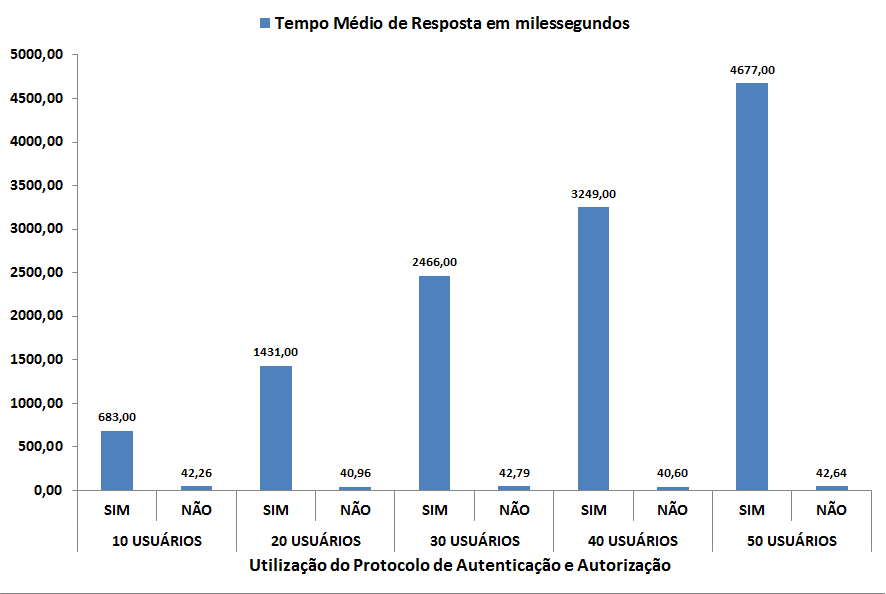
\includegraphics[width=1.0\textwidth]{grafico_teste_desempenho.png}
    \caption{Fluxo do protocolo de autenticação/autorização proposto, 1º cenário.}
    \label{fig:grafico_teste_desempenho}
\end{figure}

Para responder a segunda questão relacionada \`{a} an\'{a}lise de desemepenho (\emph{Um protótipo funcional, sem foco em otimização, consegue suportar a demanda prevista?}), 
novamente foram realizadas análises dos dados coletados nos testes realizados. A análise dos resultados obtidos com a execução do experimento ocorreu com a observação do tempo médio de resposta e com a verificação da vazão--- ou seja, o número de requisições atendidas por segundo, que foi coletado ao final da execução do Teste 10, aplicado a um grupo de 50 usuários, conforme apresentado na Tabela~\ref{tb:tb_testes}. Dessa forma, foram coletadas 5000 amostras que utilizaram o 
protocolo de autenticação e autorização proposto em um período de 11 minutos {\color{red}por que 11 minutos?}. Os resultados estatísticos são apresentados na tabela~\ref{tb:estatistica_com_cripto_50}.

Observa-se que a PCDF, em um cenário extremo, pode ter que responder a uma média de 1200 requisições de um serviço que fornece informações sobre ocorrências policiais em um período de uma hora, ou seja, duas requisições por segundo. Neste caso, os resultados obtidos com o experimento realizado com os 50 usuários, demonstrou que o tempo médio de resposta foi de 4677 milissegundos (ou aproximadamente 4,677 segundos) e que a vazão média, que é o número de requisições atendidas por segundo, foi de 8,62 requisições por segundo. Ao se realizar a comparação deste cenário com o cenário extremo vivenciado pela PCDF, verificou-se que a arquitetura, do ponto de vista de vazão, atende ao cen\'{a}rio mais cr\'{i}tico, 
que é de 2 duas requisições por segundo. O que garante a qualidade do serviço ofertado pelo protocolo de autenticação e autorização proposto.

{\color{red}essa tabela est\'{a} muito ruim. sugiro remover} 

\begin{table}[h]
\centering
\begin{tabular}{|l|l|}
\hline
\textbf{Informação} & \textbf{Valor} \\ \hline
Nº de Requisições   &  5000              \\ \hline
Média               &  4677             \\ \hline
Mínimo              &  118          \\ \hline
Máximo              &  21665        \\ \hline
Desvio Padrão       &  3170,49      \\ \hline
\% Erro             &  0,0          \\ \hline
Vazão/seg           &  8,62     \\ \hline
Kbps                &  11,8         \\ \hline
Média de Bytes      &  1401,05      \\ \hline
\end{tabular}
\caption {Estatística básica com a utilização do protocolo de autenticação e autorização para 50 usuários.}\label{tb:estatistica_com_cripto_50}
\end{table}

\section{Síntese do capítulo}

{\color{red} revisa essa s\'{i}ntese. est\'{a} furada. fala apenas do teste de desempenho} 

Neste cap\'{i}tulo foi realizada uma análise de desempenho, onde foram definidos objetivos e questões que foram respondidas após a execução e análise dos testes realizados. O estudo evidenciou que o impacto no desempenho é significativo quando comparado com a não utilização da proposta. Porém os tempos médios obtidos estão dentro de um tempo médio esperado, que é abaixo de 5 segundos. Observou-se ainda, que em um cenário extremo de utilização, onde a PCDF tenha que atender a uma média de 2 duas requisições por segundo, e um período de 1 uma hora, ou seja 1200 requisições, a arquitetura proposta atende perfeitamente, pois consegue atender a 8,62 requisições por segundo em um cenário extremo onde foram realizados 5000 requisições em aproximadamente em 10 minutos. 